% Created 2024-01-23 Tue 10:12
% Intended LaTeX compiler: pdflatex
\documentclass[presentation]{beamer}
\usepackage[utf8]{inputenc}
\usepackage[T1]{fontenc}
\usepackage{graphicx}
\usepackage{longtable}
\usepackage{wrapfig}
\usepackage{rotating}
\usepackage[normalem]{ulem}
\usepackage{amsmath}
\usepackage{amssymb}
\usepackage{capt-of}
\usepackage{hyperref}
\mode<beamer>{\usetheme{Madrid}}
\definecolor{SUred}{rgb}{0.59375, 0, 0.17969} % SU red (primary)
\definecolor{SUblue}{rgb}{0, 0.17578, 0.38281} % SU blue (secondary)
\setbeamercolor{palette primary}{bg=SUred,fg=white}
\setbeamercolor{palette secondary}{bg=SUblue,fg=white}
\setbeamercolor{palette tertiary}{bg=SUblue,fg=white}
\setbeamercolor{palette quaternary}{bg=SUblue,fg=white}
\setbeamercolor{structure}{fg=SUblue} % itemize, enumerate, etc
\setbeamercolor{section in toc}{fg=SUblue} % TOC sections
% Override palette coloring with secondary
\setbeamercolor{subsection in head/foot}{bg=SUblue,fg=white}
\setbeamercolor{date in head/foot}{bg=SUblue,fg=white}
\institute[SU]{Shenandoah University}
\titlegraphic{\includegraphics[width=0.5\textwidth]{\string~/Documents/suLogo/suLogo.pdf}}
\newcommand{\R}{\mathbb{R}}
\usepackage{tikz}
\usetheme{default}
\author{Chase Mathison\thanks{cmathiso@su.edu}}
\date{24 January 2024}
\title{Applications of Angles}
\hypersetup{
 pdfauthor={Chase Mathison},
 pdftitle={Applications of Angles},
 pdfkeywords={},
 pdfsubject={},
 pdfcreator={Emacs 29.1 (Org mode 9.6.7)}, 
 pdflang={English}}
\begin{document}

\maketitle

\section{Announcements}
\label{sec:org5619781}
\begin{frame}[label={sec:orgb99aee6}]{Announcements}
\begin{enumerate}
\item Homework in MyOpenMath!
\item Office hours canceled today.
\item Don't forget about exit tickets!
\end{enumerate}
\end{frame}

\section{Lecture}
\label{sec:org6289637}
\begin{frame}[label={sec:org138753f}]{Applied Example}
We found the radius of the earth (at the equator) in a previous example.  If this
class took place on the equator, how many miles would we rotate through over the course
of the class? (Assume I can plan well, and class takes 75 minutes).

\vspace{10in}
\end{frame}

\begin{frame}[label={sec:orgf9b2303}]{The area of a sector}
\begin{columns}
\begin{column}{0.45\columnwidth}
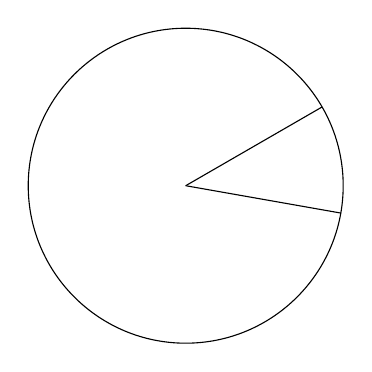
\begin{tikzpicture}
  \draw (0,0) circle [radius=2];
  \draw (0,0) -- (30:2);
  \draw (0,0) -- (-10:2);
\end{tikzpicture}
\end{column}

\begin{column}{0.45\columnwidth}
\begin{block}{Area of sector}
The area of a sector with central angle \(\theta\) of a circle of radius \(r\) is:
\vspace{1in}
\end{block}
\end{column}
\end{columns}
\end{frame}

\begin{frame}[label={sec:org25ca001}]{Linear vs angular speed}
If a wheel is spinning without slipping, one thing we might be interested in is its
\alert{angular speed}.  This is a measure of how quickly the wheel is spinning.  Your car
measures angular speed in revolutions per minute.  We'll usually use \uline{\hspace*{1in}}.

When we use radians per second to measure how fast a wheel is
spinning, it's a fun fact that you can calculate linear speed if you
know angular speed.  We'll denote angular speed with \uline{\hspace*{1in}}
and linear speed with \uline{\hspace*{1in}}.  If the wheel has radius \(r\), then
these two speeds are related by:

\[ v = \hspace{1in}\]
\end{frame}

\begin{frame}[label={sec:orgc93ab33}]{Example}
We know the radius of the earth at the equator and that Earth spins 1
time in 24 hours. Use these facts to calculate how fast (linear speed) someone
standing on the equator of the earth is going just by standing still!

\vspace{10in}
\end{frame}
\end{document}